%%%%%%%%%%%%%%%%%%%%%%%%%%%%%%%%%%%%%%%%%%%%%%%%%%%%%%%%%%
%   Autoren:
%   Prof. Dr. Bernhard Drabant
%   Prof. Dr. Dennis Pfisterer
%   Prof. Dr. Julian Reichwald
%%%%%%%%%%%%%%%%%%%%%%%%%%%%%%%%%%%%%%%%%%%%%%%%%%%%%%%%%%

%%%%%%%%%%%%%%%%%%%%%%%%%%%%%%%%%%%%%%%%%%%%%%%%%%%%%%%%%%
%	ANLEITUNG: 
%   1. Ersetzen Sie firmenlogo.jpg im Verzeichnis img
%   2. Passen Sie alle Stellen im Dokument an, die mit 
%      @stud 
%      markiert sind 
%%%%%%%%%%%%%%%%%%%%%%%%%%%%%%%%%%%%%%%%%%%%%%%%%%%%%%%%%%

%%%%%%%%%%%%%%%%%%%%%%%%%%%%%%%%%%%%%%%%%%%%%%%%%%%%%%%%%%
%	ACHTUNG: 
%   Für das Erstellen des Literaturverzeichnisses wird das 
%   modernere Paket biblatex in Kombination mit biber 
%   verwendet - nicht mehr das ältere Paket BibTex!
%
%   Bitte stellen Sie Ihre TeX-Umgebung entsprechend ein (z.B. TeXStudio): 
%   Einstellungen --> Erzeugen --> Standard Bibliographieprogramm: biber
%%%%%%%%%%%%%%%%%%%%%%%%%%%%%%%%%%%%%%%%%%%%%%%%%%%%%%%%%%

\documentclass[fontsize=11pt,BCOR=5mm,DIV=13,parskip=half,listof=totoc,
               paper=a4,toc=bibliography,pointlessnumbers]{scrreprt}



               
\usepackage[utf8]{inputenc}

%% LANGUAGE SETTINGS
%
% @stud: Sprache ggf. anpassen
%
\usepackage[english]{babel}
\usepackage{csquotes} 	% correct quoting using \enquote{}

%%%%%%%%%%%%%
%% ZITIERSTIL
%%%%%%%%%%%%%
%
% @stud: Zitierstil in package biblatex unten wählen
%
% NUMERIC Style - e. g. [12]
% style=numeric 
%
% IEEE Style - numeric kind of style 
% style=ieee 
%
% ALPHABETIC Style - e. g. [AB12]
% style=alphabetic 
%
% HARVARD Style 
% style=apa 
%
% CHICAGO Style 
%style=authoryear
%
% Position des Zitats:
%
% autocite=inline 
%
% (!!) FOOTNOTE POSITION NOT RECOMMENDED IN MINT DOMAIN:
% autocite=footnote
%
\usepackage[backend=biber, autocite=inline, style=authoryear]{biblatex} 	
\usepackage{makeidx}                  % allows index generation
\usepackage{listings}	                %Format Listings properly
\usepackage{lipsum}                   % Blindtext
\usepackage{graphicx}                 % use various graphics formats
\usepackage[english]{varioref}         % nicer references \vref
\usepackage{caption}	                % better Captions
\usepackage{booktabs}                 % nicer Tabs
\usepackage[hidelinks=true]{hyperref} % keine roten Markierungen bei Links
\usepackage{fnpct}                    % Correct superscripts 
\usepackage{calc}                     % Used for extra space below footsepline, in particular
\usepackage{array}
\usepackage{acronym}
\usepackage{algorithm}
\usepackage{algpseudocode}
\usepackage{setspace}
\usepackage{tocloft}
\usepackage[T1]{fontenc}

% Definitionen und Commands
\newcommand{\indextype}{numeric}
\newcommand{\abs}{\par\vskip 0.2cm\goodbreak\noindent}
\newcommand{\nl}{\par\noindent}
\newcommand{\mcl}[1]{\mathcal{#1}}
\newcommand{\nowrite}[1]{}
\newcommand{\NN}{{\mathbb N}}
\newcommand{\imagedir}{img}
\newcommand{\TitelDerArbeit}[1]{\def\DerTitelDerArbeit{#1}\hypersetup{pdftitle={#1}}}
\newcommand{\AutorDerArbeit}[1]{\def\DerAutorDerArbeit{#1}\hypersetup{pdfauthor={#1}}}
\newcommand{\Firma}[1]{\def\DerNameDerFirma{#1}}
\newcommand{\Kurs}[1]{\def\DieKursbezeichnung{#1}}
\newcommand{\Abteilung}[1]{\def\DerNameDerAbteilung{#1}}
\newcommand{\Studiengangsleiter}[1]{\def\DerStudiengangsleiter{#1}}
\newcommand{\WissBetreuer}[1]{\def\DerWissBetreuer{#1}}
\newcommand{\FirmenBetreuer}[1]{\def\DerFirmenBetreuer{#1}}
\newcommand{\Bearbeitungszeitraum}[1]{\def\DerBearbeitungszeitraum{#1}}
\newcommand{\Abgabedatum}[1]{\def\DasAbgabedatum{#1}}
\newcommand{\Matrikelnummer}[1]{\def\DieMatrikelnummer{#1}}
\newcommand{\Studienrichtung}[1]{\def\DieStudienrichtung{#1}}
\newcommand{\ArtDerArbeit}[1]{\def\DieArtDerArbeit{#1}}
\newcommand{\Literaturverzeichnis}{Literaturverzeichnis}

% Page Layout
%\oddsidemargin=0mm
%\evensidemargin=0mm
%\textwidth=159mm
%\topmargin=-18mm
%\headsep=10mm
%\textheight=251mm
%\footheight=15mm

\makeindex

%%%%%%%%%%%%%%%%%%%%%%%%%%%%%%%%%%%
% LITERATURVERZEICHNIS
% @stud: Literaturverzeichnis in Datei bibliography.bib anpassen. 
%
% [Alternative zu Verwendung von \initializeBibliography: Citavi ... (dazu eigenes LaTex Coding verwenden)]
%
\addbibresource{bibliography.bib}
\DefineBibliographyStrings{ngerman}{andothers = {{et\,al\adddot}},}

% Elementare Konfigurationen und Definitionen werden geladen 
% @stud: gegebenenfalls anpassen
%
% !TEX root =  master.tex

%%%%%%%%%%%%%%%%%%%%%%%%%%%%%%%%%%%%%%%%%%%%%%%%%%%%%%%%%%%%%%%%%%
%	ANLEITUNG: 
% Passen Sie gegebenenfalls alle Stellen im Dokument an, die mit 
% @stud 
% markiert sind.
%%%%%%%%%%%%%%%%%%%%%%%%%%%%%%%%%%%%%%%%%%%%%%%%%%%%%%%%%%%%%%%%%%

%%
%% @stud
%%
%% LANGUAGE SETTINGS
\usepackage[english]{babel} 	        % german language
\usepackage{csquotes} 
%\usepackage[english]{babel}          % english language
%\usepackage{csquotes} 	              % correct quoting using \enquote{}

\usepackage{makeidx}                  % allows index generation
\usepackage{listings}	                %Format Listings properly
\usepackage{lipsum}                   % Blindtext
\usepackage{graphicx}                 % use various graphics formats
\usepackage[english]{varioref}         % nicer references \vref
\usepackage{caption}	                % better Captions
\usepackage{booktabs}                 % nicer Tabs
\usepackage[hidelinks=true]{hyperref} % keine roten Markierungen bei Links
\usepackage{fnpct}                    % Correct superscripts 
\usepackage{calc}                     % Used for extra space below footsepline, in particular
\usepackage{array}
\usepackage{acronym}
\usepackage{algorithm}
\usepackage{algpseudocode}
\usepackage{setspace}
\usepackage{tocloft}
\usepackage{rotating}

%% Schriftarten- und Zeichenpakete
\usepackage[T1]{fontenc}
\usepackage[utf8]{inputenc}


%%
%% @stud
%%
%%	FONT SELECTION: Schriftarten und Schriftfamilie
%%%%%%%%%%%%%
%% SCHRIFTART
%%%%%%%%%%%%%
% 0) without decomment: normal font families 
% ...
% 1) Latin Modern 
\usepackage{lmodern}        
% 2) Times 
%\usepackage{mathptmx}         
% 3) Helvetica
%\usepackage[scaled=.92]{helvet} 
%%%%%%%%%%%%%%%%%%
%%	SCHRIFTFAMILIE
%%%%%%%%%%%%%%%%%%
% ohne Serifen
\renewcommand*{\familydefault}{\sfdefault}
\addtokomafont{disposition}{\sffamily}
%
% mit Serifen
%\renewcommand*{\familydefault}{\rmdefault}
%\addtokomafont{disposition}{\rmfamily}
%
% Typewriter
%\renewcommand*{\familydefault}{\ttdefault}
%\addtokomafont{disposition}{\ttfamily}

%%
%% @stud
%%
%% Uncomment the following lines to support hard URL breaks in bibliography 
%\apptocmd{\UrlBreaks}{\do\f\do\m}{}{}
%\setcounter{biburllcpenalty}{9000}% Kleinbuchstaben
%\setcounter{biburlucpenalty}{9000}% Großbuchstaben

%%
%% @stud
%%
%% FOOTNOTES: Count footnotes over chapters
\counterwithout{footnote}{chapter}

%	ACRONYMS
\makeatletter
\@ifpackagelater{acronym}{2015/03/20}
{\renewcommand*{\aclabelfont}[1]{\textbf{{\acsfont{#1}}}}}{}
\makeatother

%	LISTINGS
% @stud: ggf. Namen/Text anpassen (englisch)
\renewcommand{\lstlistingname}{Source Code} 
\renewcommand{\lstlistlistingname}{List of Source Codes}
\lstset{numbers=left,
	numberstyle=\tiny,
    breaklines=true,
	basicstyle=\ttfamily\small}

%	ALGORITHMS
% @stud: ggf. Namen/Text anpassen (englisch)
\renewcommand{\listalgorithmname}{Algorithmenverzeichnis}
\floatname{algorithm}{Algorithmus}

%	PAGE HEADER / FOOTER
%	Warning: There are some redefinitions throughout the master.tex-file!  DON'T CHANGE THESE REDEFINITIONS!
\RequirePackage[automark]{scrlayer-scrpage}
%alternatively with separation lines: \RequirePackage[automark,headsepline,footsepline]{scrlayer-scrpage}

\renewcommand{\chaptermarkformat}{}
\RedeclareSectionCommand[beforeskip=0pt]{chapter}
\clearpairofpagestyles

%\ifoot[\rule{0pt}{\ht\strutbox+\dp\strutbox}DHBW Mannheim]{\rule{0pt}{\ht\strutbox+\dp\strutbox}DHBW Mannheim}
\ofoot[\rule{0pt}{\ht\strutbox+\dp\strutbox}\pagemark]{\rule{0pt}{\ht\strutbox+\dp\strutbox}\pagemark}
\ohead{\headmark}

\providecommand{\TitelDerArbeit}[1]{\def\DerTitelDerArbeit{#1}\hypersetup{pdftitle={#1}}}
\providecommand{\AutorDerArbeit}[1]{\def\DerAutorDerArbeit{#1}\hypersetup{pdfauthor={#1}}}
\providecommand{\Firma}[1]{\def\DerNameDerFirma{#1}}
\providecommand{\Kurs}[1]{\def\DieKursbezeichnung{#1}}
\providecommand{\Abteilung}[1]{\def\DerNameDerAbteilung{#1}}
\providecommand{\Studiengangsleiter}[1]{\def\DerStudiengangsleiter{#1}}
\providecommand{\WissBetreuer}[1]{\def\DerWissBetreuer{#1}}
\providecommand{\FirmenBetreuer}[1]{\def\DerFirmenBetreuer{#1}}
\providecommand{\Bearbeitungszeitraum}[1]{\def\DerBearbeitungszeitraum{#1}}
\providecommand{\Abgabedatum}[1]{\def\DasAbgabedatum{#1}}
\providecommand{\Matrikelnummer}[1]{\def\DieMatrikelnummer{#1}}
\providecommand{\Studienrichtung}[1]{\def\DieStudienrichtung{#1}}
\providecommand{\ArtDerArbeit}[1]{\def\DieArtDerArbeit{#1}}
\providecommand{\Literaturverzeichnis}{Literaturverzeichnis}

\newcommand{\settingBibFootnoteCite}{
	\setlength{\bibparsep}{\parskip}		  % Add some space between biblatex entries in the bibliography
	\addbibresource{bibliography.bib}	    % Add file bibliography.bib as biblatex resource
	\DefineBibliographyStrings{english}{andothers = {{et\,al\adddot}},}
}

\newcommand{\setTitlepage}{
	% !TEX root =  master.tex
% @stud: ggf. Namen/Text anpassen (englisch)
\begin{titlepage}
    \begin{minipage}{\textwidth}
            \vspace{-2cm}
            \noindent 
\includegraphics[width=0.3\textwidth]{\imagedir/firmenlogo.jpg} \hfill 
            
\includegraphics[width=0.2\textwidth]{\imagedir/logo.jpg}
    \end{minipage}
    \vspace{1em}
    %\sffamily
    \begin{center}
        {\textsf{\textbf{\large{\DieArtDerArbeit}}}}\\[6mm]
        {\textsf{\textbf{\Large{}\DerTitelDerArbeit}}} \\[1.5cm]
        {\textsf{\textbf{\large{}Course of Study: Business Informatics}}}\\[6mm]
        {\textsf{\textbf{Specialization: \DieStudienrichtung}}}\vspace{10em}
        
        \begin{minipage}{\textwidth}
            \begin{tabbing}
            Scientific Supervisor: \hspace{0.85cm}\=\kill
            Author: \> \DerAutorDerArbeit \\[1.5mm]
            Company: \> \DerNameDerFirma  \\[1.5mm]
            Department: \> \DerNameDerAbteilung \\[1.5mm]
            Supervisor: \> \DerFirmenBetreuer \\[1.5mm]
            Company: \> SAP Labs India \\[1.5mm]
            Department: \> MD's office \\[1.5mm]
            \end{tabbing}
        \end{minipage}
        
    \end{center}
    \end{titlepage}
	\pagenumbering{roman} % Römische Seitennummerierung
	\normalfont	
}

\newcommand{\initializeText}{
	\clearpage
	\ihead{\chaptername~\thechapter} % Neue Header-Definition
	\pagenumbering{arabic}           % Arabische Seitenzahlen
}

\newcommand{\initializeBibliography}{
	\ihead{}
	\printbibliography[title=\Literaturverzeichnis] 
	\cleardoublepage
}

\newcommand{\initializeAppendix}{
	\appendix
  \ihead{}
  \cftaddtitleline{toc}{chapter}{Appendix}{}
}

% @stud
%
% PERSÖNLICHE ANGABEN (BITTE VOLLSTÄNDIG EINGEBEN zwischen den Klammern: {...})
%
\ArtDerArbeit{Whitepaper} 
\TitelDerArbeit{Creating an LLM extension for Achievements Dashboard: PoC Development for SAP Labs India}
\AutorDerArbeit{Sean Tyler Straub}
\Abteilung{Corporate IT}
\Firma{Freudenberg \& Co. KG}
\Studienrichtung{Software Engineering}
\FirmenBetreuer{Kishor Ingale}

\begin{document}

\setTitlepage


%	Kurzfassung / Abstract
% @stud: abstract.tex bearbeiten
\section*{Abstract} 
\cleardoublepage


%%%%%%%%%%%%%%%%%%%%%%%%%%%%%%%%%%%

%%%%%%%%%%%%%%%%%%%%%%%%%%%%%%%%%%%
% VERZEICHNISSE und ABSTRACT
%
% @stud: ggf. nicht benötigte Verzeichnisse auskommentieren/löschen
%
\tableofcontents
\cleardoublepage

% Abbildungsverzeichnis
%\phantomsection
%\addcontentsline{toc}{chapter}{\listfigurename}
%\listoffigures
%\cleardoublepage

%	Tabellenverzeichnis
%\phantomsection
%\addcontentsline{toc}{chapter}{\listtablename}
%\listoftables
%\cleardoublepage

%	Listingsverzeichnis / Quelltextverzeichnis
%\lstlistoflistings
%\cleardoublepage

% Algorithmenverzeichnis
% \listofalgorithms
% \cleardoublepage

% Abkürzungsverzeichnis
% @stud: acronyms.tex bearbeiten
% !TEX root =  master.tex
\clearpage
\chapter*{Acronyms}	
\addcontentsline{toc}{chapter}{Acronyms}

\begin{acronym}[XXXXXXX]	
    \acro{LLM}{Large Language Model}
    \acro{PoC}{Proof of Concept}


\end{acronym} 
\cleardoublepage

\onehalfspacing

\initializeText

%%%%%%%%%%%%%%%%%%%%%%%%%%%%%%%%%%%%%%%%%%%%%%%%%%%%%%%%%%%%%%%%%%%%%%%%%%%%%%%%%%%%%%%%%%
% KAPITEL UND ANHÄNGE
%
% @stud:
%   - nicht benötigte: auskommentieren/löschen
%   - neue: bei Bedarf hinzufügen mittels input-Kommando an entsprechender Stelle einfügen
%%%%%%%%%%%%%%%%%%%%%%%%%%%%%%%%%%%%%%%%%%%%%%%%%%%%%%%%%%%%%%%%%%%%%%%%%%%%%%%%%%%%%%%%%%

%%%%%%%%%%%%%%%%%%%%%%%%%%%%%%%%%%%
% KAPITEL
%
% @stud: einzelne Kapitel bearbeiten und eigene Kapitel hier einfügen
%

\chapter{Introduction}
\label{introduction}
\nocite{*}

\section{Background}
The \textit{Champions Circle} software at SAP Labs India is an innovative platform that recognizes and rewards employees for exceptional achievements. 
By fostering a culture of appreciation, it ensures that accomplishments across various domains, such as innovation, leadership, and diversity, are celebrated. 
However, as the software's usage grows, so does the need for an efficient and streamlined recommendation process.

The existing workflow involves multiple approval levels: from the manager, to the Leader, and finally to a jury that determines the worthiness of the achievement for the award. 
This manual process, while thorough, can be time-consuming and subject to inconsistencies. 
To address this, a \ac{PoC} was developed to integrate a \ac{LLM} extension into the \textit{Champions Circle} platform. 
This extension evaluates recommendations at the initial stage, providing a score and explanatory feedback to assist managers in their decision-making.

This paper details the \ac{PoC} development process, including the creation of a test environment to mimic the \textit{Champions Circle} software. 
This environment leveraged technologies such as \textit{Vite}, \textit{Node.js}, and \textit{HTML/JavaScript} while using SAP's categories and criteria for validation.

\section{Preread}
Before embarking on the \ac{PoC} development, it was crucial to understand the existing \textit{Champions Circle} framework and its operational workflow. 
This involved reviewing documentation shared by SAP Labs India. 

Additionally, I was provided with multiple SharePoint pages that detailed the inclusion and exclusion criteria for each category. 
I studied these criteria and simplified them into a \texttt{.csv} file, which was then used as extra information for the \ac{LLM}.

By combining insights from the \textit{Champions Circle} system and advancements in \ac{LLM} technology, the \ac{PoC} aims to enhance the recommendation process, 
ensuring fairer and more efficient evaluations.
\cleardoublepage

\chapter{Implementation}
\label{implementation}

\section{Methodology}
The objective of the \ac{PoC} was to integrate an \ac{LLM} extension into the existing \textit{Champions Circle} software to evaluate the fittingness of achievements 
before they are submitted for manager approval. The process aimed to simplify and enhance the recommendation workflow by providing managers with a score (1-10) and an 
explanation of why the achievement is suitable for the nominated category. To achieve this, the following methodology was followed:

\begin{enumerate}
    \item \textbf{Understanding the Existing System:} The first step was to review the existing \textit{Champions Circle} software and its operational workflow. 
    This involved understanding how recommendations are made for various achievement categories, 
    and the roles and responsibilities of the participants in the approval process (Manager, Leader, Jury).
    
    \item \textbf{Defining Criteria for Evaluation:} As part of the \ac{PoC}, additional criteria were defined for the \ac{LLM} to consider when evaluating the fittingness of achievements. 
    These criteria were derived from multiple SharePoint pages shared by SAP Labs India, detailing the inclusion and exclusion rules for each category. 
    These rules were compiled into a \texttt{.csv} file, which was used as supplementary input to the \ac{LLM}.
    
    \item \textbf{Creating a Test Environment:} Since direct access to the internal codebase of the \textit{Champions Circle} application was unavailable, a test environment was created. 
    Using Vite, HTML, JavaScript, and a Node.js server, a web-based version of the application was developed to simulate the process of achievement recommendations. 
    This environment was used to integrate and test the \ac{LLM} extension.
    
    \item \textbf{Integrating the \ac{LLM}:} The \ac{LLM} was integrated into the test application with the task of evaluating the achievements before they are submitted to the manager. 
    The \ac{LLM} utilized the simplified \texttt{.csv} files containing categories and additional criteria, which allowed it to assess each achievement according to the defined rules. 
    The output of the \ac{LLM} included a score between 1 and 10, alongside an explanation of why the achievement fit the given category.
    
    \item \textbf{Simulating the Workflow:} The test environment simulated the workflow of the original \textit{Champions Circle} application, 
    with the \ac{LLM} providing recommendations and feedback. 
    The results were displayed to the manager in a way that simplified their approval process by showing both the score and the reasoning behind it.
\end{enumerate}

\section{Implementation}
The implementation of the \ac{PoC} involved several key components, including the development of the test environment, the integration of the \ac{LLM}, 
and the configuration of the \texttt{.csv} files for categories, criteria, and questions.

\begin{enumerate}
    \item \textbf{Web-Based Test Application:} A web-based prototype was developed using Vite for rapid development, with HTML, CSS, and JavaScript used for the frontend. 
    The backend was powered by a Node.js server, which facilitated interactions with the \ac{LLM} and managed the achievement evaluation process.
    
    \item \textbf{Category and Criteria Files:} Predefined categories, including Process Innovation, Product Innovation, Enablement, Rising Star, Industry Thought Leader, Organizational Thought Leader, 
    Customer Centricity, Purpose, and Diversity and Inclusion, were provided in a \texttt{.csv} file. Another \texttt{.csv} file was created to outline the inclusion and exclusion criteria for each category, 
    ensuring the \ac{LLM} could evaluate achievements accurately. When an achievement was submitted, the application sent the relevant category and criteria to the \ac{LLM} for evaluation. 
    For example, the Enablement category's criteria are detailed in the Listing~\ref{lst:enablement_criteria}.    
    
    \begin{lstlisting}[caption={Evaluation Criteria Enablement}, label={lst:enablement_criteria}]
        Category Evaluation Criteria:
          - **Inclusions**: Training conducted over and above your regular work requirements: we consider the following under this category: d-Shop, SAP TechEd and SAP d-com, Learning Fest, Going beyond your day to day responsibilities to enable customers/stakeholders about the industry/product. Mentoring conducted over and above your regular work requirements. We consider the following under this category: Coached/Mentored employees under central initiatives: Invent for Customers, IE Summit, etc., Mentoring under the global Mentorship program
          - **Exclusions**: Inter/Intra team trainings do not count as a contribution under this category. Coaching/Mentoring a new joinee within the team does not count as a contribution under this category.
    \end{lstlisting}
    
    \item \textbf{Questions:} A second \texttt{.csv} file was provided which contained predefined questions, each associated with a specific category. 
    These questions were designed to help clarify and define the achievement, ensuring that the \ac{LLM} could better assess the fittingness of the achievement for the corresponding category.
    
    \item \textbf{Integration of the \ac{LLM}:} The \ac{LLM} was integrated into the application through the Node.js server, 
    which allowed the web application to send achievement details along with the relevant parts of the \texttt{.csv} files to the \ac{LLM} for evaluation. 
    The \ac{LLM} processed these inputs and returned a score with pass or fail, accompanied by an explanation, which was then displayed to the user.

    \item \textbf{Prompt Engineering:} The system prompt was refined throughout the development process to ensure that passing and failing grades were selected with good accuracy. 
    The final iteration resulted in the system prompt shown in \ref{lst:evaluation_instructions}.
\end{enumerate}

\section{Examples}
\label{examples}

This section provides a walkthrough of the functionality and outcomes of the \ac{PoC}, demonstrating how the web-based application interacts with the \ac{LLM} for achievement evaluation. 
Screenshots of the application interface and results are included to illustrate the workflow.

\subsection{Category Selection and Dynamic Questions}
The application allows users to select a category from a dropdown menu. Based on the selected category, relevant questions dynamically populate the page to guide the user in defining their achievement. 
Figure~\ref{fig:categories} shows the dropdown menu with available categories, and Figure~\ref{fig:empty} provides an overview of the initial page for the "Enablement" category, 
showcasing the first few dynamically generated questions.

\begin{figure}[H]
    \centering
    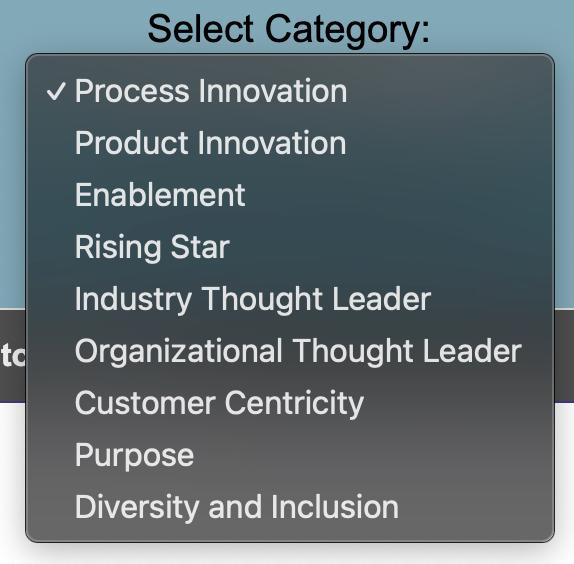
\includegraphics[width=0.5\textwidth]{img/categories.jpeg}
    \caption{Dropdown menu for selecting a category.}
    \label{fig:categories}
\end{figure}

\begin{figure}[H]
    \centering
    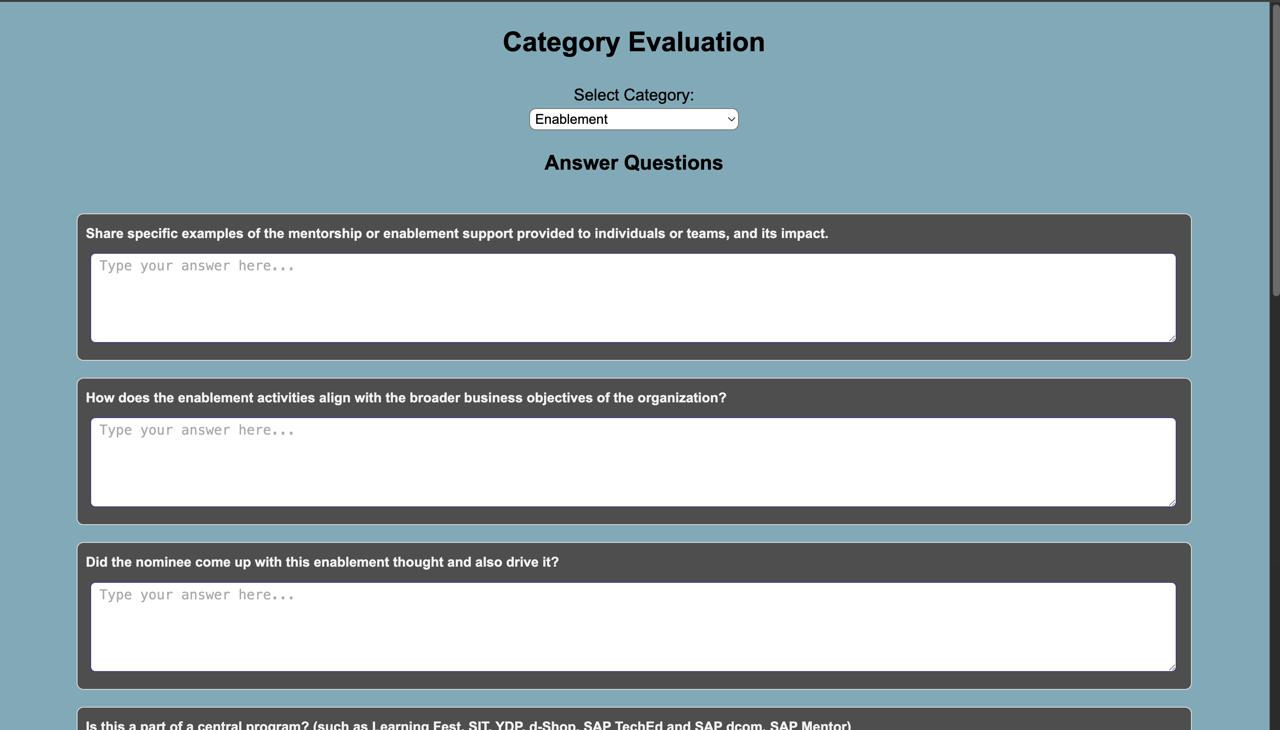
\includegraphics[width=0.9\textwidth]{img/empty.jpeg}
    \caption{Initial view of the page with the "Enablement" category selected.}
    \label{fig:empty}
\end{figure}

\subsection{Questionnaire Completion and Submission}
Once the user has answered all questions, they can submit their responses for evaluation. 
Figure~\ref{fig:submit} shows the bottom of the page, where the last few questions are answered and the "Submit" button is displayed.

\begin{figure}[H]
    \centering
    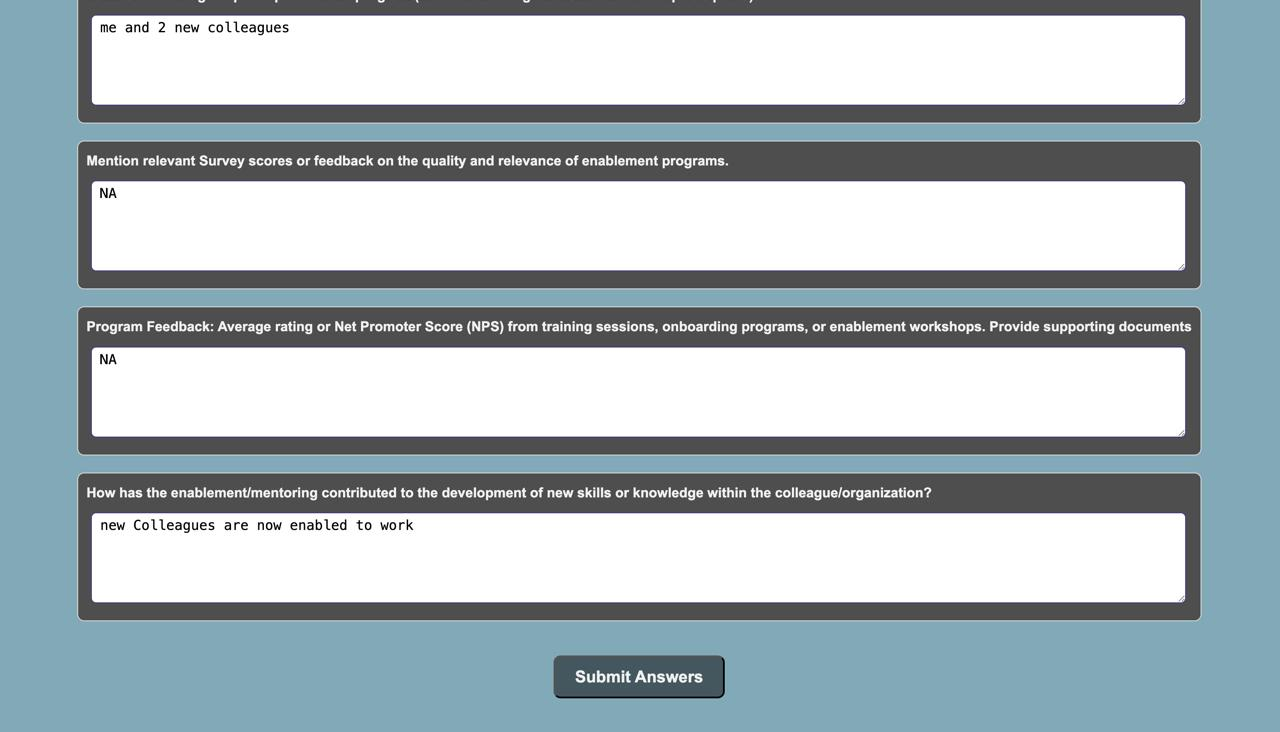
\includegraphics[width=0.9\textwidth]{img/submit.jpeg}
    \caption{Final view of the questionnaire before submission.}
    \label{fig:submit}
\end{figure}

\subsection{Evaluation Outcomes}
After submission, the \ac{LLM} evaluates the achievement based on the criteria defined for the selected category. 
Two examples are provided below, demonstrating both a failed and a successful submission for the "Enablement" category.

\subsubsection{Failed Submission}
Figure~\ref{fig:fail} shows the evaluation result for a failed submission. The achievement failed with a score of 3 due to not meeting the inclusion criteria and falling under the exclusion criteria. 
As specified in Listing~\ref{lst:enablement_criteria}, intra-team training and coaching a new joinee are excluded from consideration for this category.

\begin{figure}[H]
    \centering
    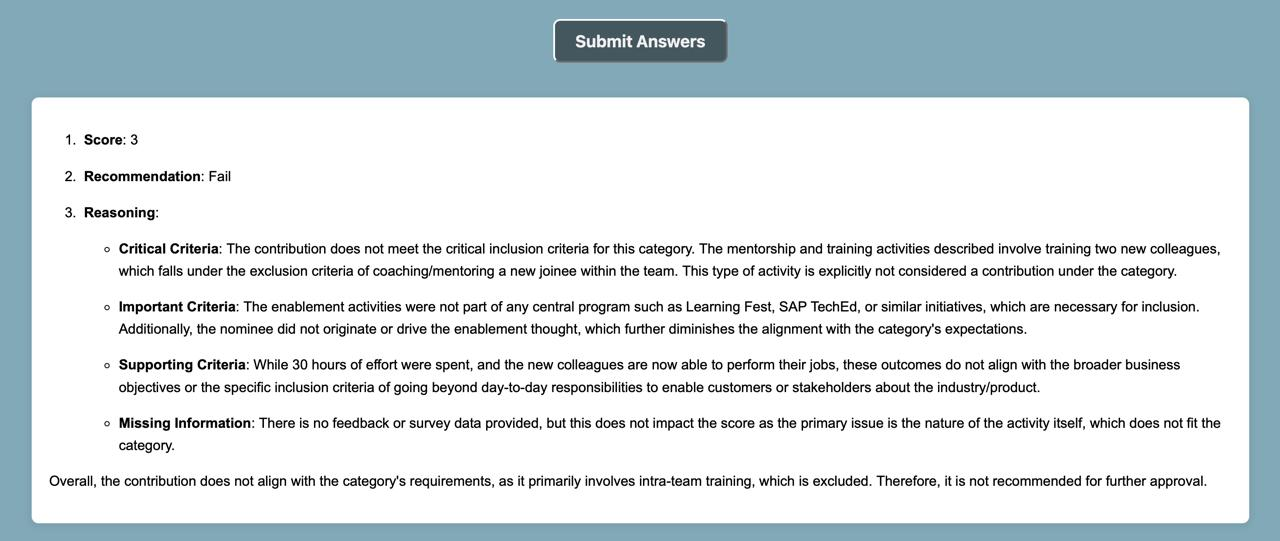
\includegraphics[width=0.9\textwidth]{img/fail.jpeg}
    \caption{Evaluation result for a failed submission under the "Enablement" category.}
    \label{fig:fail}
\end{figure}

\subsubsection{Successful Submission}
In contrast, Figure~\ref{fig:pass} shows a successful submission for the "Enablement" category. The achievement scored 7 and received a "Pass" recommendation. 
This submission involved creating worksheets and assisting with a Young Developers Program (YDP) event, aligning with the inclusion criteria. 
Additional factors that contributed positively were the nominee's 15 hours of effort and positive feedback received.

\begin{figure}[H]
    \centering
    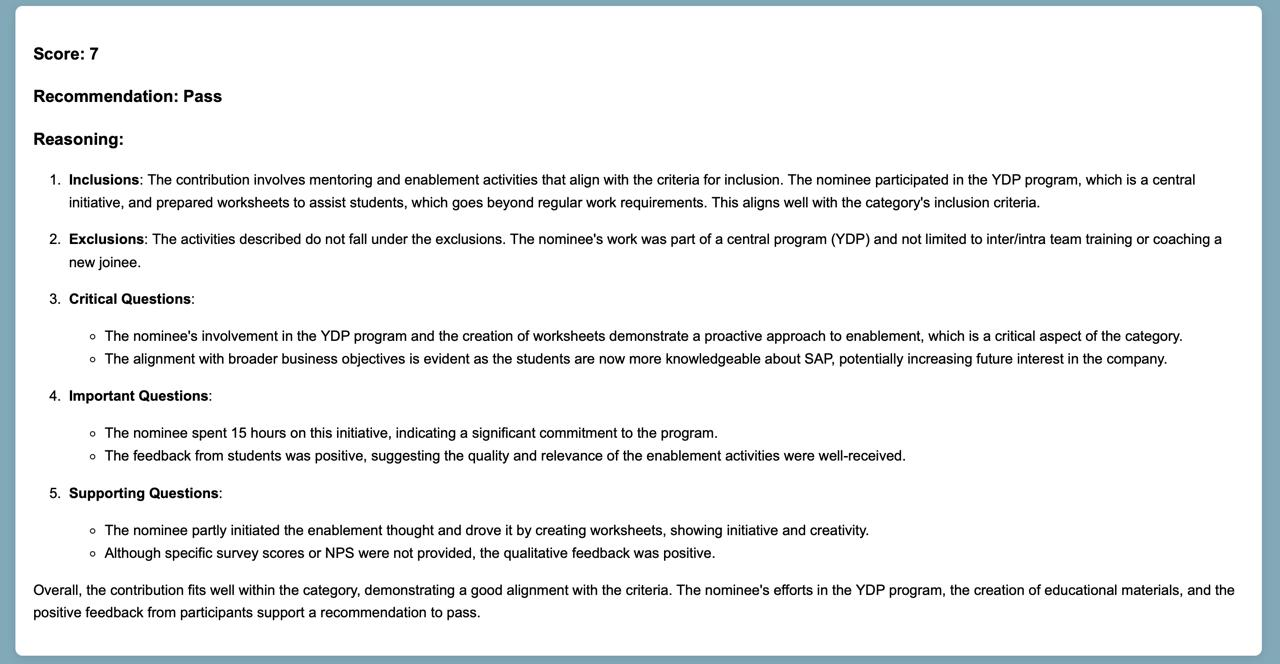
\includegraphics[width=0.9\textwidth]{img/pass.jpeg}
    \caption{Evaluation result for a successful submission under the "Enablement" category.}
    \label{fig:pass}
\end{figure}

\subsection{Prompt Debugging}
For transparency and debugging purposes, the application logs the user prompt sent to the \ac{LLM}. Figure~\ref{fig:prompt} displays the terminal output for the successful submission, 
showing the evaluation criteria, questions, and user responses. Note that the system prompt used during evaluation can be found in Listing~\ref{lst:evaluation_instructions}.

\begin{figure}[H]
    \centering
    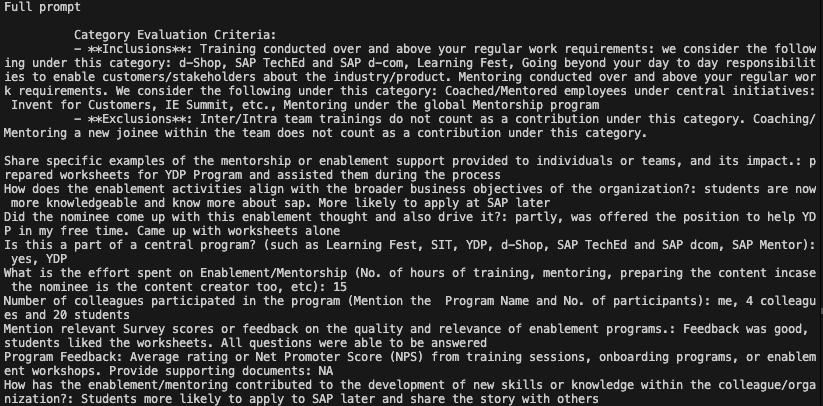
\includegraphics[width=0.9\textwidth]{img/prompt.jpeg}
    \caption{Terminal output showing the user prompt for a successful submission.}
    \label{fig:prompt}
\end{figure}
\cleardoublepage

\chapter{Conclusion}
\label{conclusion}

The \ac{PoC} demonstrated the feasibility of integrating an \ac{LLM} into an achievement evaluation process, leveraging dynamic questionnaires and predefined criteria for robust assessments. 
This chapter summarizes the findings and outlines potential next steps to further refine and expand the implementation.

\section{Findings}
The development and testing of the \ac{PoC} yielded several key findings:
\begin{itemize}
    \item The integration of the \ac{LLM} with dynamic category-based questionnaires effectively streamlined the evaluation process, providing actionable recommendations with detailed explanations.
    \item Predefined inclusion and exclusion criteria stored in \texttt{.csv} files were instrumental in ensuring consistent evaluations aligned with organizational goals.
    \item Prompt engineering played a critical role in refining the \ac{LLM}'s responses. Iterative improvements to the system prompt resulted in more accurate evaluations of achievements.
    \item Testing identified the impact of user answers, category-specific criteria, and prompt settings on the evaluation outcomes, highlighting areas for further optimization.
\end{itemize}

\section{Next Steps}
Building on the success of the \ac{PoC}, the following steps are recommended for advancing this project:

\subsection*{Expanding Criteria}
Additional inclusion and exclusion criteria should be added to the \texttt{.csv} files to cover a broader range of categories and scenarios. 
This will improve the versatility of the system and ensure it meets diverse organizational needs.

\subsection*{Integration into UI5 and CAP}
The current web-based prototype needs to be adapted into a full-fledged implementation using SAP UI5 and CAP to integrate seamlessly with the existing corporate website. 
This transition will align the solution with the organization's technology stack and enhance scalability.

\subsection*{Refining Prompt Engineering}
Further iterations of prompt engineering should be conducted to maximize the accuracy and reliability of the \ac{LLM}'s evaluations. 
This includes experimenting with different temperature settings to determine the optimal balance between creativity and consistency in responses.

\subsection*{Comprehensive Testing}
Additional testing is necessary to validate the system across various edge cases and categories. 
This includes stress testing the application with large datasets and diverse achievements to ensure consistent performance and reliability.

\subsection*{User Feedback and Iterative Improvement}
Incorporating feedback from end-users will be vital for refining the system's usability and effectiveness. 
Iterative improvements based on user insights will ensure the solution aligns with real-world expectations and requirements.

These next steps will transform the \ac{PoC} into a robust and scalable system, providing a valuable tool for achievement evaluation and recognition within the organization.

\cleardoublepage
%%%%%%%%%%%%%%%%%%%%%%%%%%%%%%%%%%%

%%%%%%%%%%%%%%%%%%%%%%%%%%%%%%%%%%%
% ANHÄNGE
%
% @stud: einzelne Anhänge bearbeiten und eigene Anhänge hier einfügen 
%        die nachfolgenden Zeilen deaktivieren, wenn keine Anhänge verwendet werden
%
\initializeAppendix
\chapter{System Prompt Engineering}
\label{appendix}

\begin{lstlisting}[caption={Prompt Engineering Evaluation Instructions}, label={lst:evaluation_instructions}]
    role: "system",
      content: `
You are an expert evaluator assessing the relevance and quality of a contribution for a specific category at SAP Labs India. Follow these instructions and respond in Markdown format:\n

### Instructions:\n
1. **Evaluation Criteria**: Assess the contribution based on the provided **criteria** (inclusions and exclusions).\n
2. **Weighting Questions**:\n
   - Weigh critical questions more heavily than others.\n
   - Do not assign equal importance to all questions; prioritize the ones that are most critical.\n
3. **Scoring**: Assign a single cumulative score from 1 to 10:\n
   - **1**: Does not fit the category at all.\n
   - **10**: Perfectly fits the category.\n
   "- Use the full scoring range: \n  - 0-3: The contribution does not fit the category.\n  
   - 4-6: The contribution fits the category but is not strong or impactful.\n  
   - 7-9: The contribution is good and aligns well with the category.\n  
   - 10: The contribution is exceptional and demonstrates excellence in one or more aspects."\n
4. **Recommendation**:\n
   - Clearly state whether the contribution should **pass** (recommended for manager approval) or **fail** (not recommended for further approval).\n
5. **Structured Reasoning**:\n
   - Justify your score by referencing specific answers to critical, important, and supporting questions.\n
   - Explicitly link your reasoning to the criteria and responses provided.\n
6. **Missing Answers**:\n
   - Missing answers should not reduce the score but indicate insufficient information for specific aspects.\n
7. **Restrictions**:\n
   - **Do not** provide feedback on question quality.\n
   - **Do not** suggest improvements to the contribution or process.\n

### Response Format:\n
1. **Score**: [Score from 1 to 10]\n
2. **Recommendation**: [Pass/Fail]\n
3. **Reasoning**: [Structured explanation referencing criteria and responses]`,
    },
    {
      role: "user",
      content: `
### Criteria:\n
${criteriaText}
\n
### Responses to Questions:\n
${prompt}
`,
\end{lstlisting}

% \input{appendix2}
%%%%%%%%%%%%%%%%%%%%%%%%%%%%%%%%%%%

\singlespacing

\setlength{\bibitemsep}{1.5em}

%\ihead{}
%\printbibliography[title=\Literaturverzeichnis] 
%\printbibliography 
%\cleardoublepage

%\initializeBibliography
%%%%%%%%%%%%%%%%%%%%%%%%%%%%%%%%%%%

%%%%%%%%%%%%%%%%%%%%%%%%%%%%%%%%%%%
% INDEX
% @stud: ggf. Index auskommentieren, wenn nicht benötigt
%
% \addcontentsline{toc}{chapter}{Index}
% \printindex

\end{document}